\subsection{Software Architecture Requirements} \label{software_requirements}

Figure \ref{fig_design} illustrates the generic software architecture of the artifacts.
Each instantiated element adheres to the Element Naming Convention outlined in Appendix
\ref{appendix_element_naming_convention}. The following tables detail the requirements
specific to each element.

\begin{figure}[H]
    \centering
    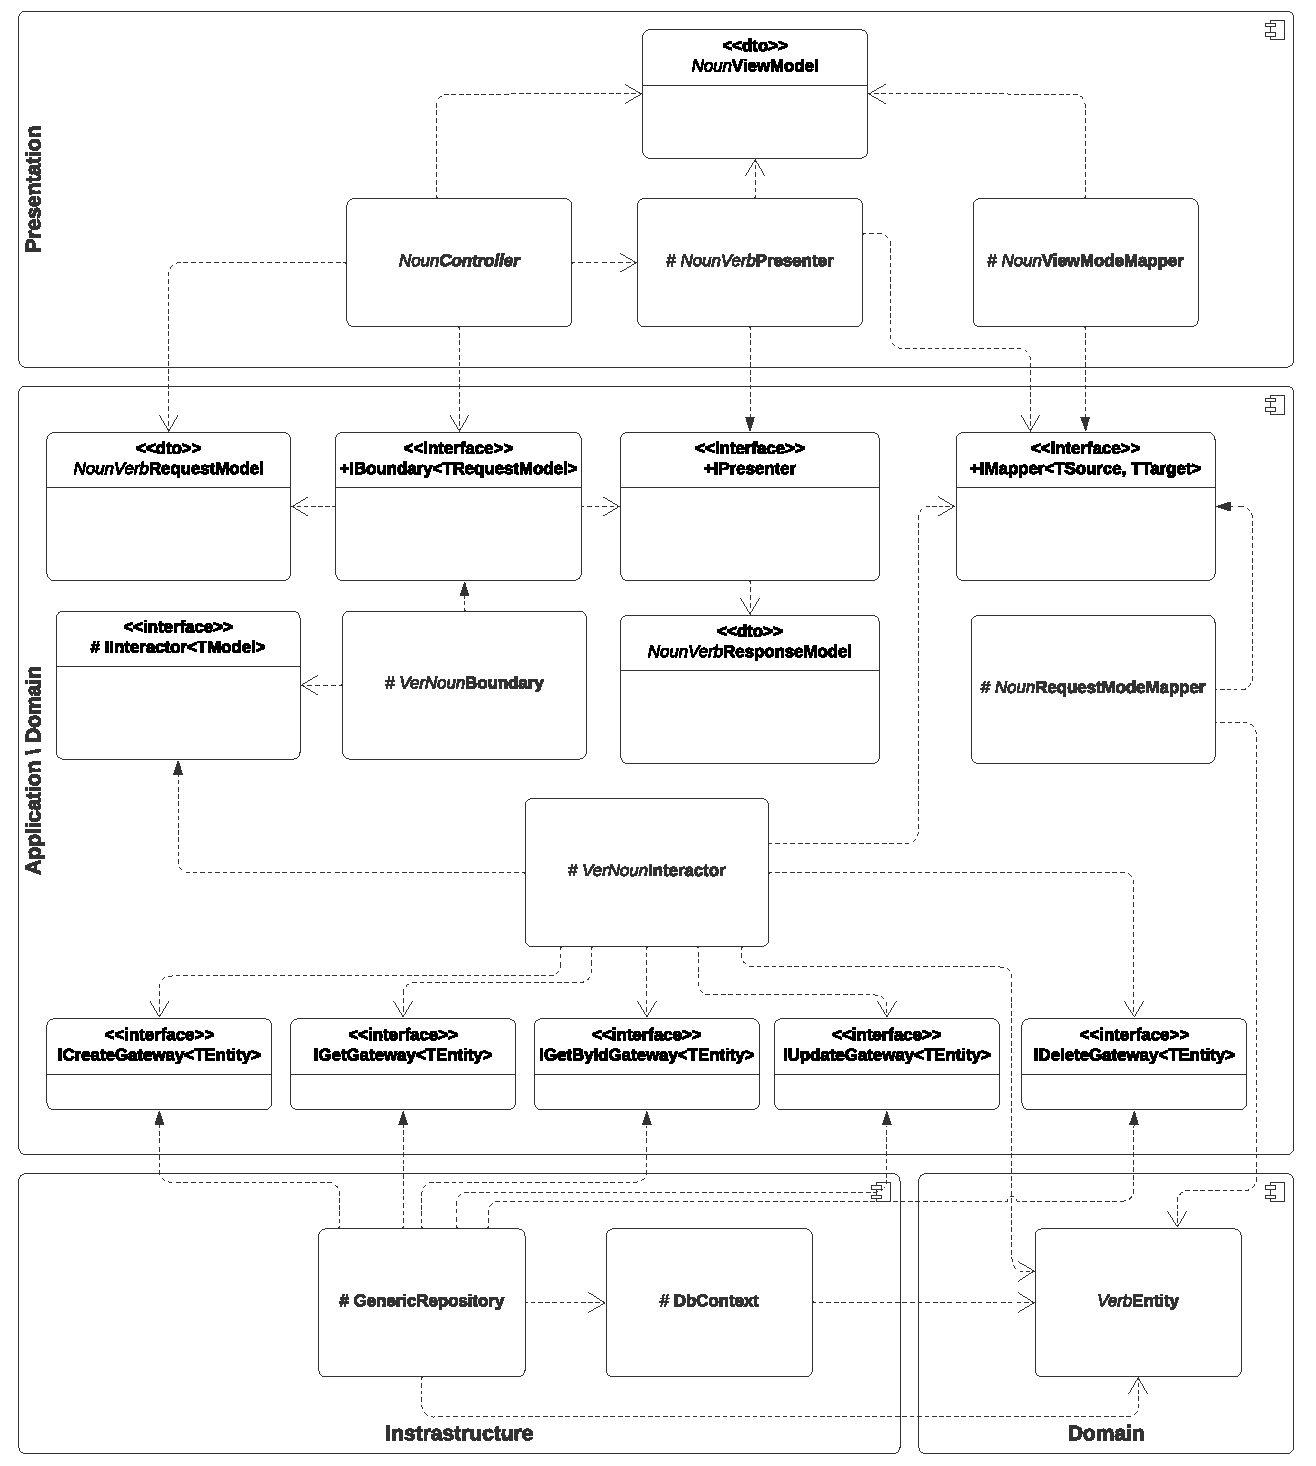
\includegraphics[width=1\textwidth]{figures/generic_design.pdf}
    \caption[Generic architecture]{The Generic architecture of the artifacts}
    \label{fig_design}
\end{figure}

\requirement{The ViewModel}{table_requirements_viewmodel}{
    
    \addEvalRow{The ViewModel consists of data attributes representing fields from the
    corresponding Entity. In addition, it may contain information specific to the user
    interface.}

    \addEvalRow{The ViewModel has no external dependencies on other objects within the
    architecture.}
}

\requirement{The Presenter}{table_requirements_presenter}{

    \addEvalRow{The Presenter Implementation is derived from the IPresenter interface and follows the
    specified implementation. The IPresenter interface can be found in the Application
    layer.}
    
    \addEvalRow{The Presenter is responsible for creating the Controller's Response by instantiating
    the ViewModel, constructing the HTTP Response message, or combining both elements as
    needed.}
    
    \addEvalRow{When required, the Presenter utilizes the IMapper interface without depending on
    specific implementations of the IMapper interface.}
    
    \addEvalRow{The Presenter has an internal scope and cannot be instantiated outside the
    Presentation layer.} }


\requirement{The ViewModelMapper}{table_requirements_viewModelMapper}{

    \addEvalRow{The ViewModelMapper is derived from the IMapper interface and follows the specified
    implementation. The IMapper interface can be found in the Application layer.}

    \addEvalRow{The ViewModelMapper is responsible for mapping the values of the necessary data
    attributes from the ResponseModel to the ViewModel.}
    
    \addEvalRow{The ViewModelMapper has an internal scope and cannot be instantiated
    outside the Presentation layer.} }

\requirement{The Controller}{table_requirements_controlle}{

    \addEvalRow{The Controller is responsible for receiving external requests and forwarding the
    request to the appropriate Boundary within the Application layer.}

    \addEvalRow{The Controller relies on the IBoundary interface without depending on specific
    implementations of the IBoundary interface.}
}

\subsubsection*{The Application Layer}


\requirement{The IBoundary}{table_requirements_iboundary}{

    \addEvalRow{The IBoundary interface establishes the contract for its derived Boundary implementations.}

    \addEvalRow{The IBoundary interface has public scope within the system.}
}

\requirement{The Boundary Implementation}{table_requirements_boundary}{

    \addEvalRow{A Boundary implementation is derived from the IBoundary interface and follows the
    specified implementation.}

    \addEvalRow{The Boundary implementation separates the internal aspects of the
    Application Layer and the other layers within the component.}
    
    \addEvalRow{Each Boundary implementation handles a single task, executed using the IInteractor interface.}
    
    \addEvalRow{Boundary implementations have an internal scope and cannot be instantiated outside the
    Application layer.}
}

\requirement{The IInteractor}{table_requirements_iinteractor}{

    \addEvalRow{The IInteractor interface establishes the contract for its derived Interactor
    implementations.}

    \addEvalRow{The IInteractor has an internal scope and cannot be implemented outside the Application
    layer.}
}

\requirement{The Interactor Implementation}{table_requirements_interactor}{

    \addEvalRow{An Interactor implementation is derived from the IInteractor interface and follows the
    specified implementation.}

    \addEvalRow{The Interactor implementation executes a single task or orchestrates a series of
    tasks. Each of these tasks is implemented in separate Interactors. Alternatively, a
    Gateway is used for Tasks with Infrastructure dependencies, such as data persistence
    in a database.}

    \addEvalRow{ Depending on the task, the Interactor implementation orchestrates the mapping from
    RequestModels to Entities or from Entities to ResponseModels, utilizing the IMapper
    interface. }

    \addEvalRow{Interactor implementations have an internal scope and cannot be implemented outside
    the Application layer.}
}

\requirement{The IMapper}{table_requirements_imapper}{

    \addEvalRow{The IMapper interface establishes the contract for its derived Mapper implementations.}

    \addEvalRow{The IMapper interface has a public scope within the system.}
}

\requirement{The RequestModelMapper}{table_requirements_requestmodelmapper}{

    \addEvalRow{The RequestModelMapper is derived from the IMapper interface and follows the specified
    implementation.}

    \addEvalRow{The RequestModelMapper is responsible for mapping the values of the necessary data
    attributes from the RequestModel to an Entity.}

    \addEvalRow{The RequestModelMapper has an internal scope and cannot be implemented outside
    the Application layer.}
}

\requirement{The ResponseModelMapper}{table_requirements_responsemodelmapper}{

    \addEvalRow{The RequestModelMapper is derived from the IMapper interface and follows the specified
    implementation.}

    \addEvalRow{The RequestModelMapper is responsible for mapping the values of the necessary data
    attributes from the RequestModel to an Entity.}

    \addEvalRow{The RequestModelMapper has an internal scope and cannot be implemented outside the
    Application layer.}
}

\requirement{The IPresenter}{table_requirements_ipresenter}{

    \addEvalRow{The IPresenter interface establishes the contract for its derived Presenter
    implementations, typically implemented as part of the Presentation layer.}

    \addEvalRow{The IPresenter interface has a public scope within the system.}
}

\requirement{The Gateway}{table_requirements_IGateway}{ \addEvalRow{The Domain and Application
    layers have no dependencies on infrastructure technologies, like web- or database
    technologies. }

    \addEvalRow{The \textit{[Verb]Gateway} interface establishes the contract for its derived Gateway
    implementations, typically implemented in the Infrastructure layer.}

    \addEvalRow{The \textit{[Verb]}Gateway interface has a public scope within the system.}

    \addEvalRow{Each task is represented in the naming convention of the interface. For
    example, the basic CRUD actions result in five IGateway interfaces:  ICreateGateway,
    IGetGateway, IGetByIdGateway, IUpdateGateway, and IDeleteGateway.} }

\requirement{The ResponseModel}{table_requirements_responsemodel}{

    \addEvalRow{The ResponseModel consists primarily of data attributes representing the fields of the
    corresponding Entity. Additionally, the ResponseModel may contain data specific to the
    output of the Interactor.}

    \addEvalRow{The ResponseModel does not depend on external objects within the architecture.}
}

\requirement{The RequestModel}{table_requirements_requestmodel}{

    \addEvalRow{The RequestModel consists primarily of data attributes representing the fields of the
    corresponding Entity. Additionally, the RequestModel may contain data specific to the
    input of the Interactor.}

    \addEvalRow{The RequestModel does not depend on external objects within the architecture.}
}

\subsubsection*{The Domain Layer}
\requirement{The Data Entity}{table_requirements_data_entity}{

    \addEvalRow{The Data Entity consists solely of attributes representing the corresponding data
    fields.}

    \addEvalRow{The Data Entity does not rely on external objects within the architecture.}

    \addEvalRow{The Application layer is the only layer that utilizes the Data Entity.}
}

\subsubsection*{The Infrastructure Layer}

\requirement{The Gateway Implementation}{table_requirements_gatewayimplementation}{

    \addEvalRow{The [\textit{Verb}]Gateway Implementation derives from the I[\textit{Verb}]Gateway interface
    and adheres to the specified implementation.}

    \addEvalRow{The [\textit{Verb}]Gateway Implementation is responsible for the interaction
    associated with the specific task, utilizing the infrastructure technology of the
    specific layer (e.g., a SQL database or a filesystem).}

    \addEvalRow{The [\textit{Verb}]Gateway Implementation has an internal scope and cannot be
    instantiated outside the layer.}
}

\subsubsection*{Design Principles Compliance}

\requirement{The Design Principles}{table_design_principles}{

    \addEvalRow{Each architectural pattern adheres to at least one of the SOLID principles to ensure that
    none of the implementations violate these principles.}
}
